\section{The RISC-V Open Source ISA}
RISC-V is the fifth generation of RISC processors, which have been in development since the 1980s at the University of California at Berkeley. Hence the name RISC-V has the ``five'' spelled out as a Roman numeral. One cannot talk about RISC-V's history without mentioning that of the MIPS ISA, which began in the same timeframe at Stanford in the 1980s. While MIPS was very popular in its own right, RISC was the inspiration for many ISAs including Sun Microsystems’ SPARC line, DEC’s Alpha line, Intel’s i860 and i960 processors, and indeed the ARM processors that most of us now carry in our pockets.

RISC-V is by no means the first open source ISA. Sun Microsystems introduced the OpenSPARC project in 2005 using the GNU Public License (GPL)\cite{anemaet2003microprocessor}. As many students of SoC architecture classes will know, the MIPS architecture was provided under an ``open use'' license in a pilot program by Wave Computing allowing its use in educational settings without licensing fees. ARM has partly opened its architecture allowing specific partners to proposed changes to the ISA they license. Many of these changes in industry practices reflect a growing need for openness in hardware. As Asanovi{\'c} notes, ``While instruction set architectures (ISAs) may be proprietary for historical or business reasons, there is no good technical reason for the lack of free, open ISAs'' \cite{asanovic2014instruction}. RISC-V is also not an example of open source hardware as there is nothing inherent in the specifications encouraging the end product to be non-proprietary. However, it is certainly an enabler for open source hardware development by facilitating the sharing of ideas in the form of ISA extensions and hardware tooling.

Care must be taken not to assume that the value found in open source software can be simply replicated in the hardware world. However, there is value to be gained for certain, and many of the same foundations underpinning open source software development as well as many of the lessons learned by those communities can be applied in hardware. Red Hat's Patent Promise and the growing problem that international regulations introduce are just two examples \cite{amye2021}. The fundamental concept of extensibility is perhaps the most obvious cross-cutting concern between open source hardware and software. Tim O'Reilly mentions the importance of extensibility to the proliferation of open source software 1990's. As O'Reilly notes, ``According to Linus Torvalds, Linux has succeeded at least in part because it followed good design principles, which allowed it to be extended in ways that he didn’t envision when he started work on the kernel. Similarly, Larry Wall explains how he created Perl in such a way that its feature-set could evolve naturally, as human languages evolve, in response to the needs of its users.'' \cite{o1999lessons}. Key to RISC-V's success will be the proliferation of open source extensions, tools, and designs that anyone can use as a platform on which to produce and launch innovative hardware.

RISC-V \gls{pmp} is developed as part of the ``TEE Task Group'' of RISC-V International. While membership in RISC-V International is required to participate in the development of specifications, membership is free for individuals and open to anyone. Specifications are developed using public mailing lists, and a review of each specification is open to a public review period before ratification. The specifications themselves are stored on a public GitHub repository where anyone can view the text during its development. RISC-V PMP was added to the Privileged ISA Specification \cite{PrivIsa2019} in 2019. Several libraries have been introduced to take advantage of this technology including: Multizone \cite{pinto2019industry}, Sanctum \cite{Costan2016a}, TIMBER-V \cite{weiser2019timber}, Mi6 \cite{bourgeat2019mi6}, and Keystone Enclave \cite{lee2019keystone, lee2020keystone, cheangverifying}. We will concentrate on Keystone Enclave as it is open source and still in active development.

\section{The RISC-V Memory Model}
RISC-V hardware threads, which are referred to in the specification as ``harts'' \cite{UnprivIsa2019}, have a byte-addressable address space of 2\textsuperscript{XLEN} bytes for all memory accesses. Here, XLEN refers to the width of a register in either 32 or 64 bits. Words are defined as having 32 bits. Halfwords are 16 bits, doublewords are 64 bits (8 bytes), and so on. The address space can be thought of as a ring, so that the last memory address is adjacent to the first. Memory instructions will simply wrap around the space ignoring that they have effectively ``walked off the end''. The specification leaves room for virtual memory by allowing for both explicit and implicit stores and loads. Chapter 3 defines the ``Zifencei'' extension, which defines a fence instruction that explicitly synchronizes writes to instruction memory and instruction fetches on the same \gls{hart}. The order in which these loads and stores happen is up to the implementation, and the rules for consistency are defined in the memory model.

The memory model of an instruction set architecture defines the values returned by a load. The main memory model for RISC-V is the \gls{rvwmo} model, ``which is designed to provide flexibility for architects to build high-performance scalable designs while simultaneously supporting a tractable programming model'' \cite{UnprivIsa2019}. There is also the ``Ztso'' extension which gives us the RISC-V Total Store Ordering (RVTSO) memory consistency model. One can think of RVTSO as the ``stronger'' model when compared to \gls{rvwmo}. We will only cover \gls{rvwmo} briefly here as knowledge of RVTSO is not required to understand \gls{pmp}, nor is a deep understanding of the \gls{rvwmo} required.

The microarchitecture implementing any given memory model is only required by the architecture to follow the memory model rules set forth in the model. This model does not set any other regulation on how the implementation achieves those rules, be the implementation speculative or not, in order or out of order, multithreaded or not, etc. As such, the \gls{rvwmo} starts by defining a set of primitives it uses to define the model. The base primitives are load and store, defined in Chapter 8 which covers the ``A'' Standard Extension for Atomic Instructions \cite{UnprivIsa2019}. It then uses a combination of \gls{axiomatic} and \gls{operational} semantics to define how memory consistency should be achieved.

The memory model defines the syntactic dependencies of memory operations. This is essentially a way to understand what the differences are between memory operations and the instructions which generate those operations. The memory model then defines thirteen rules that allow for the program order of each \gls{hart} to be consistent with the global order of all operations, called the ``preserved program order''. The rules cover overlapping address ordering, explicit synchronization, syntactic dependencies, and pipeline dependencies. The model then defines three axioms: the Load Value Axiom, the Atomicity Axiom, and the Progress Axiom. Any implementation which follows the \gls{rvwmo} memory model must conform to the thirteen rules and satisfy the three axioms.

\section{RISC-V Physical Memory Attributes}
RISC-V system's physical memory map has various properties and capabilities that are described in detail in the Privileged Specification \cite{PrivIsa2019} and referred to as \gls{pma}. These attributes determine things like read, write, and execute permissions of a specific region of physical memory. Most systems build on the RISC-V architecture will require that the \glspl{pma} are checked later in the pipeline and that this check is done in hardware. This is in contrast to other architectures where these types of checks are done in virtual page tables where the \gls{tlb} contains the information the pipeline needs regarding these attributes. RISC-V systems call the mechanism for making these checks the ``\gls{pma} checker'' and many physical attributes will be hardwired into the checker when designing the chip. For those attributes that are not known at design time there are special platform specific control registers that can be configured at runtime.

Memory regions are given attributes based on if they are part of main memory or part of I/O. The access width of a region can be anything from 8-bit byte to long multi-word bursts. As the specification states, ``Complex atomic memory operations on a single memory word or doubleword are performed with the
load-reserved (LR) and store-conditional (SC) instructions.'' \cite{PrivIsa2019}. RISC-V also allows for special \glspl{amo} which are instructions that perform operations for multiprocessor synchronization. A given \gls{pma} will contain information regarding which atomic operations are allowed for a specific region of memory.  Table \ref{table:riscv-pma-amo} lists the \gls{amo} available to I/O as of this writing.

\renewcommand{\arraystretch}{1.5}
\begin{table*}[htp]
\begin{center}
\begin{tabular}{|l|l|}
  \hline
  AMO Class & Supported Operations \\
  \hline
  AMONone       & {\em None} \\
  AMOSwap       & {\tt amoswap} \\
  AMOLogical    & above + {\tt amoand}, {\tt amoor}, {\tt amoxor} \\
  AMOArithmetic & above + {\tt amoadd}, {\tt amomin}, {\tt amomax}, {\tt amominu}, {\tt amomaxu} \\
  \hline
\end{tabular}
\end{center}
\caption[RISC-V Atomic Instructions for I/O]{\textbf{Classes of AMOs supported by I/O regions.} Reproduced from the original RISC-V Privileged Specification \cite{PrivIsa2019}.}
\label{table:riscv-pma-amo}
\end{table*}

As mentioned earlier, regions of memory will be classified either as main memory or as I/O, and this must be considered by the FENCE instruction when ordering memory. Regardless of if the memory model used is \gls{rvwmo} or RVTSO, memory regions may be classified as either having relaxed or strong ordering. Strongly ordered memory regions use a ``channel'' mechanism to guarantee ordering. Using \glspl{pma}, systems can decide to set the type of ordering dynamically or not. The specification requires that all regions of memory be coherent, such that any change made by one agent to a memory region must eventually be visible other agents of the system. Cacheability is left up to the platforms, however three types are called out: ``master-private, shared, and slave-private'' \cite{PrivIsa2019}. \glspl{pma} will describe the specific cache features of each region as well as if the region is idempotent.

\section{RISC-V Physical Memory Protection}
Unlike \glspl{pma}, RISC-V \glsreset{pmp}\gls{pmp} consists of a set of configurations that can be changed dynamically during runtime. The privileged specification describes a ``\gls{pmp} unit'' as a set of ``per-hart machine-mode control registers to allow physical memory access privileges (read, write, execute) to be specified for each physical memory region.'' \cite{PrivIsa2019}. These registers must be checked in parallel with the \gls{pma} attributes described int he previous section.

\renewcommand{\arraystretch}{2}
\begin{table}[t]
\centering
\begin{tabular}{|l|l|l|}
\hline
\textbf{Processor Mode} & \textbf{Description} \\ \hline
U Mode & User Processor Mode \\ \hline
S Mode & Supervisor Processor Mode \\ \hline
H Mode & Hypervisor Processor Mode (Draft) \\ \hline
M Mode & Machine Processor Mode \\ \hline
\end{tabular}
\caption[RISC-V Processor Modes]{\textbf{RISC-V Privilege Level Mapping} is similar to Arm's exception level mapping in that we have four modes. The most privileged machine mode is the only required mode.}
\label{table:rv-priv}
\end{table}


As we discussed in the last two chapters, processor privilege levels or ``modes'' are a critical foundation to our security model. RISC-V \gls{pmp} allows for specific registers that are only available to the highest privileged machine-mode or m-mode. The different processor modes for RISC-V are described briefly in Table \ref{table:rv-priv}. Note that H Mode is still only in the draft state, and is not applicable when discussing \gls{pmp}. While \gls{pmp} is available in both 64 bit and 32 bit versions, we will only describe 32 bit configurations in this thesis. It is enough for our comparison that we understand that a 64 bit implementation is possible and holds to the same or better standards as the 32 bit version. 

\renewcommand{\arraystretch}{1}
\vspace{.1cm}
\begin{figure}[hpt]
{\footnotesize
\adjustbox{minipage=1.3em,valign=t}{\subcaption{}\label{sfig:pmpcfg}}
\begin{subfigure}[b]{\textwidth}
\begin{center}
\begin{tabular}{@{}Y@{}Y@{}Y@{}Yl}
\instbitrange{31}{24} &
\instbitrange{23}{16} &
\instbitrange{15}{8} &
\instbitrange{7}{0} & \\
\cline{1-4}
\multicolumn{1}{|c|}{pmp3cfg} &
\multicolumn{1}{c|}{pmp2cfg} &
\multicolumn{1}{c|}{pmp1cfg} &
\multicolumn{1}{c|}{pmp0cfg} &
\tt pmpcfg0 \\
\cline{1-4}
8 & 8 & 8 & 8 & \\
\instbitrange{31}{24} &
\instbitrange{23}{16} &
\instbitrange{15}{8} &
\instbitrange{7}{0} & \\
\cline{1-4}
\multicolumn{1}{|c|}{pmp7cfg} &
\multicolumn{1}{c|}{pmp6cfg} &
\multicolumn{1}{c|}{pmp5cfg} &
\multicolumn{1}{c|}{pmp4cfg} &
\tt pmpcfg1 \\
\cline{1-4}
8 & 8 & 8 & 8 & \\
\instbitrange{31}{24} &
\instbitrange{23}{16} &
\instbitrange{15}{8} &
\instbitrange{7}{0} & \\
\cline{1-4}
\multicolumn{1}{|c|}{pmp11cfg} &
\multicolumn{1}{c|}{pmp10cfg} &
\multicolumn{1}{c|}{pmp9cfg} &
\multicolumn{1}{c|}{pmp8cfg} &
\tt pmpcfg2 \\
\cline{1-4}
8 & 8 & 8 & 8 & \\
\instbitrange{31}{24} &
\instbitrange{23}{16} &
\instbitrange{15}{8} &
\instbitrange{7}{0} & \\
\cline{1-4}
\multicolumn{1}{|c|}{pmp15cfg} &
\multicolumn{1}{c|}{pmp14cfg} &
\multicolumn{1}{c|}{pmp13cfg} &
\multicolumn{1}{c|}{pmp12cfg} &
\tt pmpcfg3 \\
\cline{1-4}
8 & 8 & 8 & 8 & \\
\end{tabular}
\end{center}
\end{subfigure}
}
{\footnotesize
\adjustbox{minipage=1.3em,valign=t}{\subcaption{}\label{sfig:pmpaddr}}
\begin{subfigure}[b]{\textwidth}
\begin{center}
\begin{tabular}{@{}J}
\instbitrange{31}{0} \\
\hline
\multicolumn{1}{|c|}{address[33:2] (\warl)} \\
\hline
32 \\
\end{tabular}
\end{center}
\end{subfigure}
}
{\footnotesize
\adjustbox{minipage=1.3em,valign=t}{\subcaption{}\label{sfig:pmpcfglayout}}
\begin{subfigure}[b]{\textwidth}
\begin{center}
\resizebox{.85\textwidth}{!}{
\begin{tabular}{YSSYYY}
\instbit{7} &
\instbitrange{6}{5} &
\instbitrange{4}{3} &
\instbit{2} &
\instbit{1} &
\instbit{0} \\
\hline
\multicolumn{1}{|c|}{L (\warl)} &
\multicolumn{1}{c|}{\wiri} &
\multicolumn{1}{c|}{A (\warl)} &
\multicolumn{1}{c|}{X (\warl)} &
\multicolumn{1}{c|}{W (\warl)} &
\multicolumn{1}{c|}{R (\warl)}
\\
\hline
1 & 2 & 2 & 1 & 1 & 1 \\
\end{tabular}
}
\end{center}
\end{subfigure}
}
\caption[RISC-V 32 bit PMP CSR Layout and Format]{\textbf{RV32 PMP CSR layout and format as well as the address register format.} Figure \ref{sfig:pmpcfg} describes the RV32 PMP configuration CSR layout. Figure \ref{sfig:pmpaddr} is the PMP address register format for RV32. Lastly, Figure \ref{sfig:pmpcfglayout} shows the PMP configuration register format. Figures reproduced from the RISC-V privileged specification \cite{PrivIsa2019}.}
\label{fig:pmpcfg-rv32}
\end{figure}

There are currently up to 16 \gls{pmp} configuration registers available in both 32 and 64 bit modes and their layout for 32 bit is shown in Figure \ref{fig:pmpcfg-rv32}. The figure also describes the layout of those configuration registers where\;\warl\;is Write-Any Read-Legal and\;\wiri\;is Write-Ignored Read-Ignored. This is to say that the two bits 5 and 6 are simply ignored in this register as they are reserved. All the other bits will follow the RISC-V common\;\warl\;as defined in the CSR section of the specification. There is also an address register format defined in Figure \ref{fig:pmpcfg-rv32}, which is the starting address of the \gls{pmp} region. No ``stop address'' is required, and if only one \gls{pmp} region is defined, it will encompass the entire memory space. Indeed when many systems boot they may choose to create a single \gls{pmp} region with read/write/execute enabled for all modes as a default setting.

The ``L'' bit of the configuration register defines if that region of memory is locked and cannot be read, written, or executed from, regardless of the processor mode. A reset is required for m-mode to once again control that CSR and allow that region's permissions to change. As mentioned, bits 6 and 5 are reserved. Bits 4 and 3 define the type of address matching scheme that will be used to match the store or load address range against the \gls{pmp} address register. The options for this two bit value are OFF, Top of Range (TOR), Naturally Aligned 4-byte region (NA4), or Naturally Aligned Power of Two (NAPOT). If set to NAPOT the granularity can be set by the system to any NAPOT value greater than or equal to 8. The last three bits are set to 1 or 0 for read, write, and execute, with 1 meaning ``enabled'' and 0 meaning ``disabled''. These bits currently apply to both S Mode and U Mode, though we will discuss the future of S Mode \gls{pmp} in a following section.

Using these configuration registers and address registers, RISC-V systems are able to create regions of memory with simple read, write, and execute privileges enforced by hardware. This allows systems to build secured areas of memory similar to that of both Intel \gls{sgx} and Arm TrustZone. However, without a framework on which to build these secured areas of memory, the specification only enables hardware engineers to create a foundation on which to build a \gls{tee}. We will now examine Keystone Enclave, an open source framework for building hardware \glspl{tee} using RISC-V \gls{pmp} as the foundation.

\section{Keystone Enclave}
One of the first \gls{tee} solutions for RISC-V \gls{pmp} came out of the MIT Computer Science \& Artificial Intelligence Laboratory (CSAIL) and a project called Sanctum \cite{Costan2016a}. This work was done just before the RISC-V \gls{pmp} task group ratified the first version of their specification for \gls{pmp} in 2017. As such it was more of a prototype and required non-standard extensions to the RISC-V core. Keystone Enclave came out of efforts of researchers at UC Berkeley and takes advantage of the ratified \gls{pmp} specification.

As detailed in Figure \ref{figure:keystone-overview}, Keystone is a full software stack containing a firmware base which launches both trusted and untrusted runtimes. These runtimes then launch both trusted, isolated applications into the enclave as well as untrusted applications into the user space of a Linux-based operating system. Keystone defines a set of \gls{tee} primitives \cite{lee2020keystone}: Secure Boot, a ``Secure Source of Randomness'', and Remote Attestation. Keystone builds its framework off these primitives and allows for customization of their firmware which they call a secure monitor (SM). The SM is used to ``enforce TEE guarantees on the platform'' \cite{lee2019keystone}, and does so by taking advantage of key proprieties of RISC-V machine mode. These properties include machine mode's programability, its ability to delegate interupts, and its ability to manage memory access using \gls{pmp}.

\begin{figure}[h]
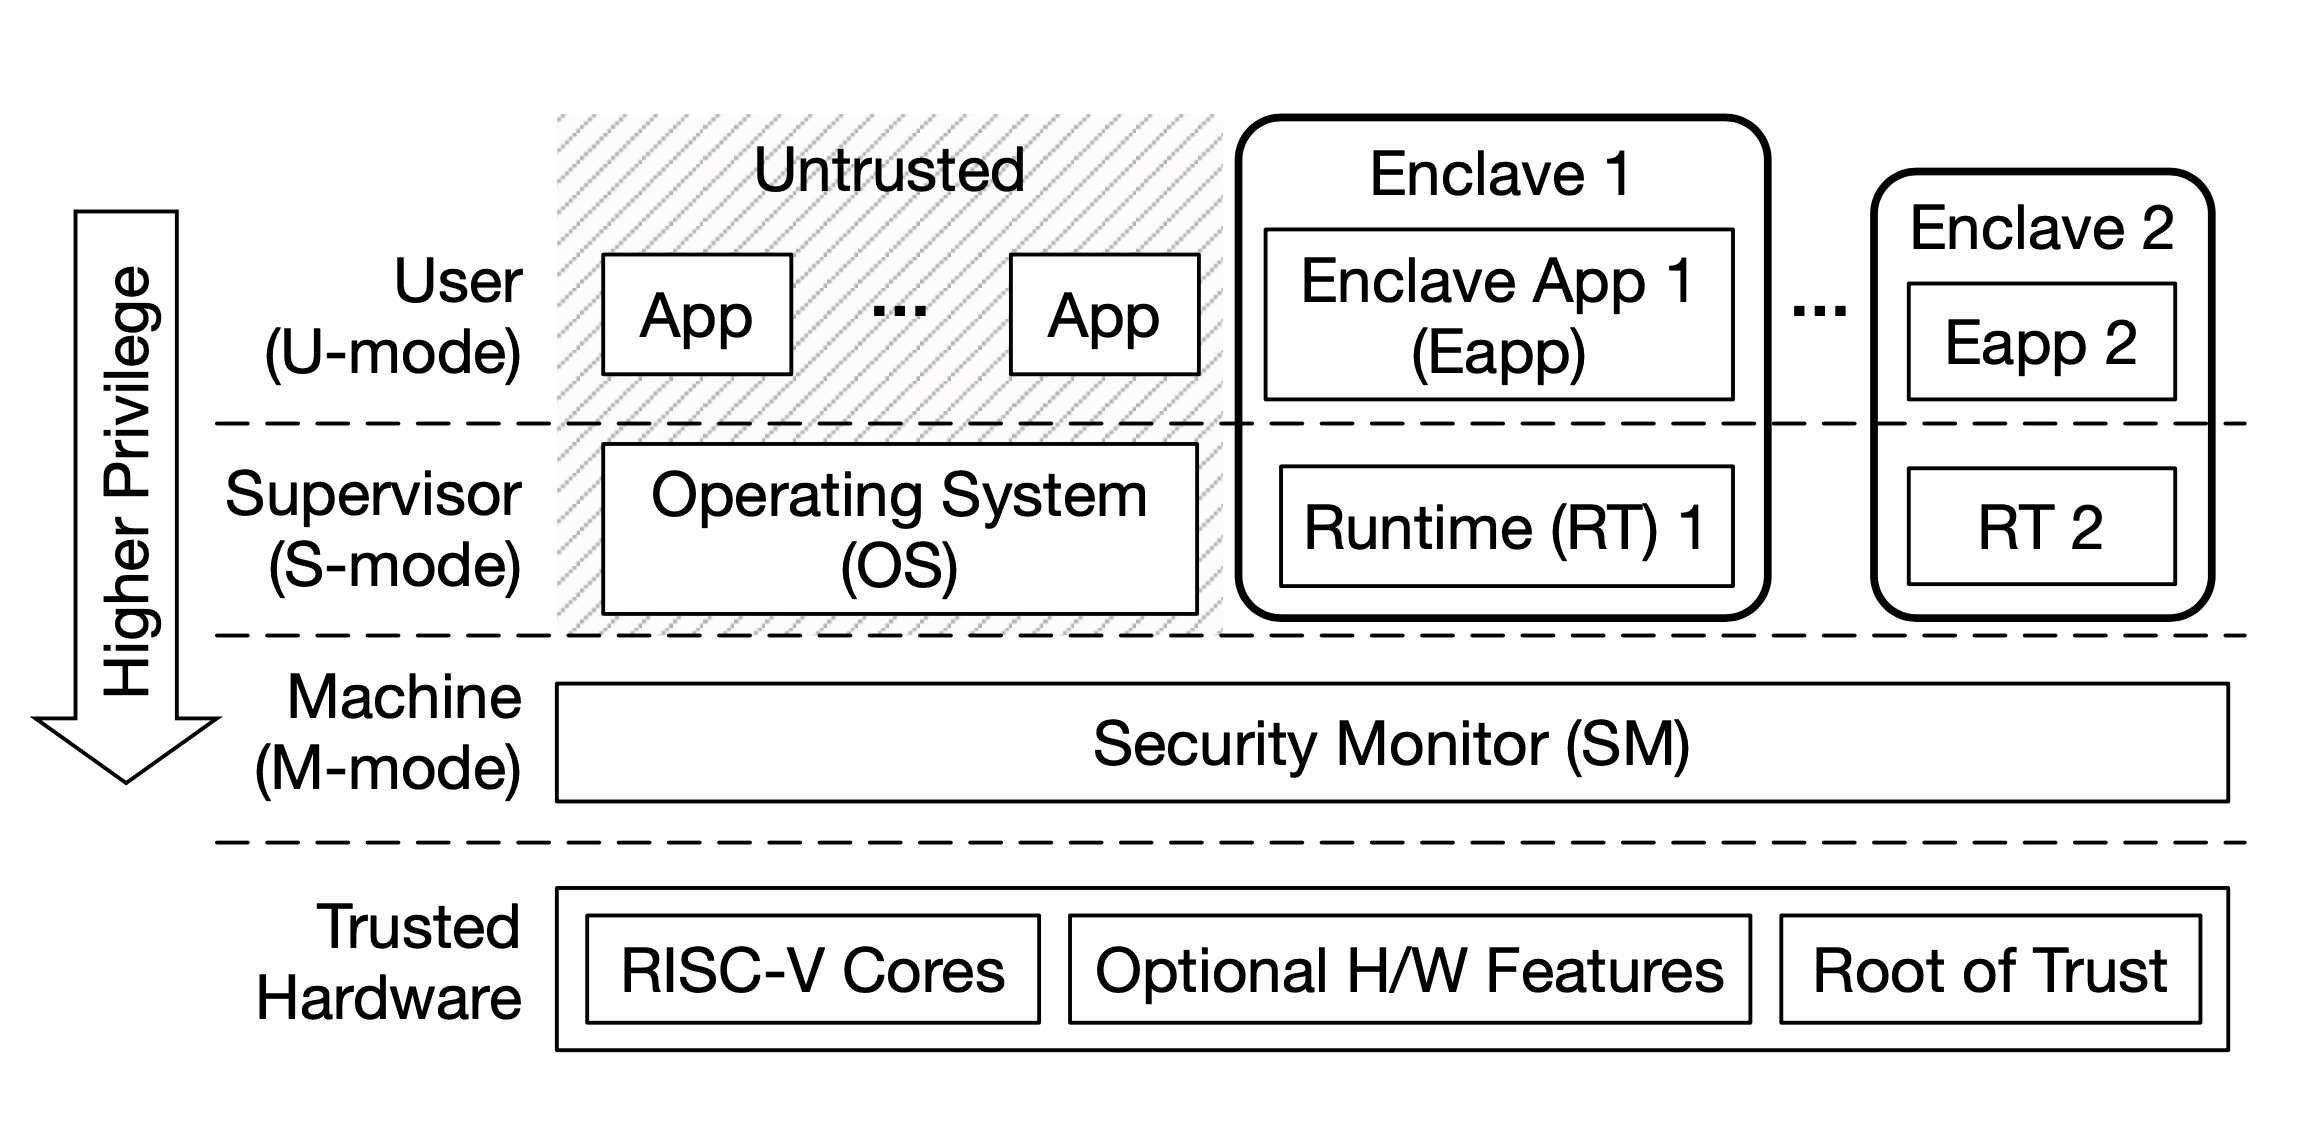
\includegraphics[width=\textwidth]{img/keystone-diagram-tmp.png}
\caption[Keystone System Overview]{\textbf{A high level overview of a Keystone Enclave system.} The Keystone codebase includes the security monitor, enclave runtime, enclave application, Linux as an untrusted OS, and untrusted host applications. Reprinted as a simplified version from Figure 1 \cite{lee2019keystone}.
\label{figure:keystone-overview}}
\end{figure}

There are two key features of RISC-V \gls{pmp} which Keystone takes advantage of in building their framework. The first is memory isolation which allows the secure monitor (SM) running in machine mode to restrict access to the enclave's memory. The second feature is the ability for \gls{pmp} to allow Keystone Enclave secure applications to use multiple hardware threads in executing code. As Lee notes, ``RISC-V provides per-hardware-thread views of physical memory via machine-mode and PMP registers. Using RISC-V thus allows multiple concurrent and potentially multi-threaded enclaves to access disjoint memory partitions while also opening up supervisor-mode and the MMU for enclave use.'' \cite{lee2020keystone}. 

\begin{figure}[h]
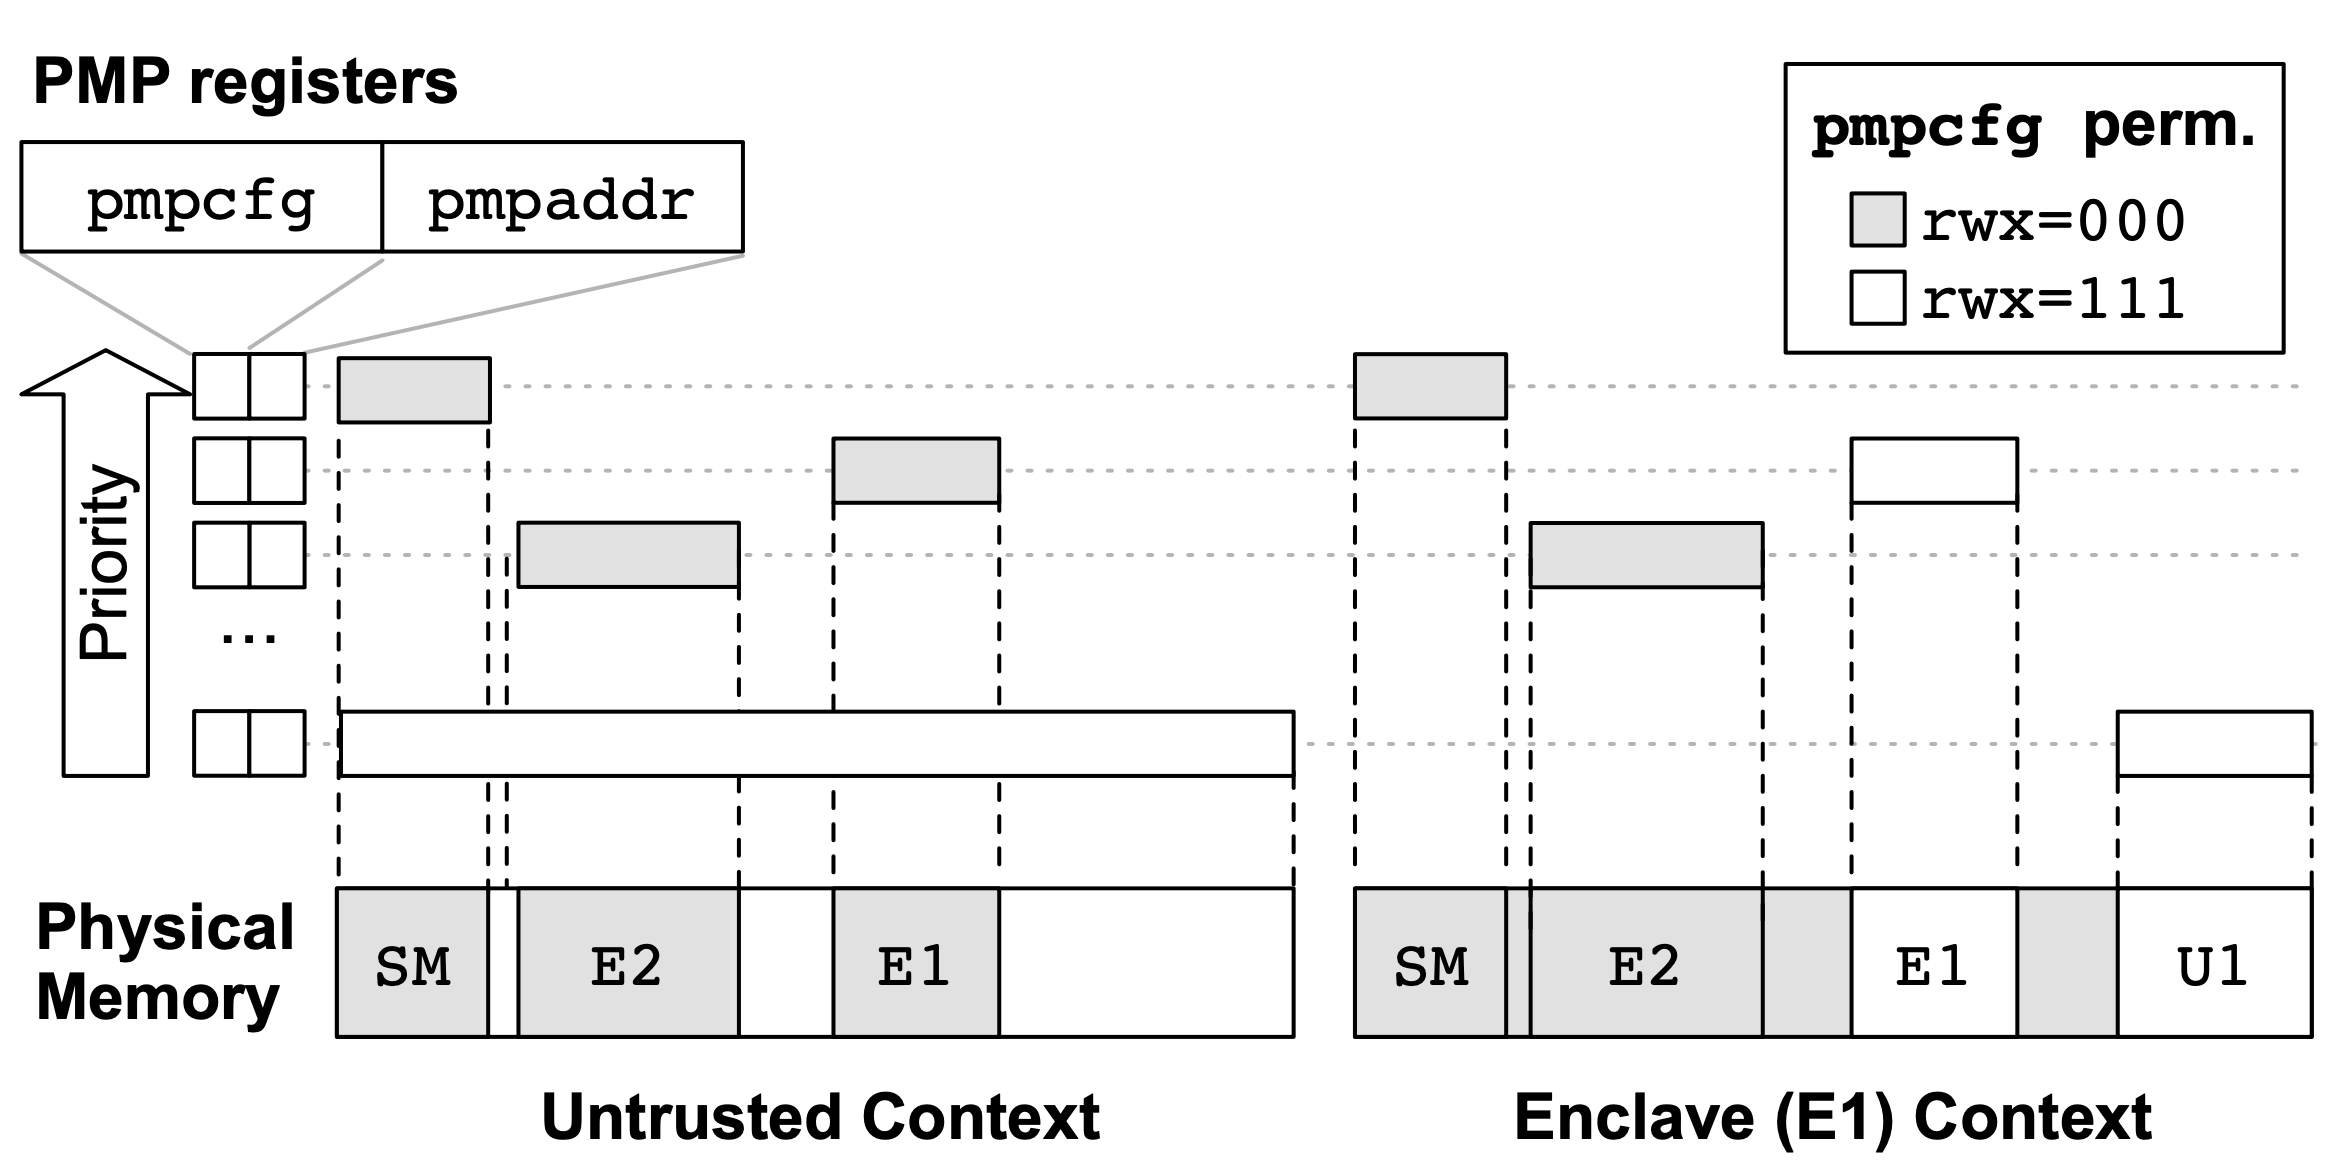
\includegraphics[width=\textwidth]{img/keystone-pmp-tmp.png}
\caption[Keystone PMP Protection]{\textbf{Keystone memory isolation using RISC-V PMP as a primitive.} Keystone separates each untrusted and trusted application into its own memory space. The secure monitor (SM) is responsible for ensuring that the proper pmpcfg and pmpaddr configurations are applied with the correct permissions. Reprinted as a simplified version from Figure 2 \cite{lee2019keystone}.
\label{figure:keystone-pmp}}
\end{figure}

Looking at Figure \ref{figure:keystone-pmp}, we can see the way in which Keystone Enclave restricts access to several sections of memory. Keep in mind that the priority of these regions are read from top to bottom with the top being the highest priority and the bottom the lowest. In the untrusted context a lowest priority area is created in order to give read, write, and execute permission to both supervisor and user modes. This allows the untrusted os, in this case Linux, to run applications anywhere outside the secure monitor and enclave regions. The security monitor sets its own region configuration as the highest priority such that no other code should be allowed access to the secure monitor's region. When a context switch is made into machine mode (E1 Context), the processor begins executing enclave code. The secure monitor switches the enclave (E1) and user application (U1) configuration bits. Those regions of memory now have read, write, and execute privileges until the context switches back to the ``Untrusted Context''. 

The memory management of these enclaves is controlled by the Keystone Enclave runtime called ``Eyrie'' which can be seen in the high level diagram in Figure \ref{figure:keystone-overview} as RT1 and RT2. Eyrie runs in Supervisor Mode and not only performs page table operations, but also allows for dynamically resizing the enclave. The security monitor has a plugin which allows for pages which must be evicted from secure memory to be encrypted such that the integrity of the data can be assured as it leaves the trusted region. This pluggable interface of the secure monitor and Eyrie runtime, along with the open source nature of the project as a whole, allows for great flexibility. For example, the secure monitor has an ``on-chip memory plugin'' \cite{lee2019keystone} that allows for use of a scratchpad memory onto which the enclave can be loaded. The Eyrie runtime has a plugin which allows an enclave to communicate with host applications in a secure manner using a shared buffer. While syscalls are not allowed inside the enclave itself, the secure monitor can either proxy those syscalls to the untrusted application, or run them in a trusted context if appropriate (e.g. mmap, brk, getrandom) \cite{lee2019keystone}.

While Keystone Enclave provides many features that we require in our definition of a \gls{tee}, some features are notably left to the user. Remote attestation is possible, however as the Keystone authors note, ``Key distribution, revocation, attestation services, and anonymous attestation are orthogonal challenges'' \cite{lee2019keystone}. There are projects currently working on the problem of remote attestation on RISC-V hardware \cite{shepherd2021lira}, however these efforts are still in their infancy. Keystone Enclaves provide a method of local attestation which makes use of provisioned keys. Enclaves can, during runtime, request signed attestation from the secure monitor in a kind of attestation report similar to that found in Sanctum \cite{lebedev2018secure}. This local attestation is built off of a Secure Boot process that is very similar to TrustZone's model, and includes the use of hardware key management and cryptographic engines. Efforts to continue work on secure boot RISC-V systems is the focus of research \cite{haj2019lightweight}, but no dominant technology currently exists as a de facto standard.

\section{Future Extensions of RISC-V Memory Protection}

There are several additional features of RISC-V \gls{pmp} that will doubtless play a role in future work done on Keystone Enclave or any RISC-V based \gls{tee} framework.